% chap3.tex (Implementation)

\chapter{Implementation}\label{IMPL-CHAP}
In section \ref{sec:pd}, I discussed the different problems I need to solve and in chapter \ref{BACK-CHAP}, I have discussed the different tools and technologies I used in this thesis. Here, I will talk about how I solved those problems using said tools, particularly the implementation details of each individual components or events (e.g., testbed setup, traffic generation), and will describe the execution workflow of the emulation.

\begin{figure}[H]
	\begin{center}
		\resizebox{\textwidth}{!}
		{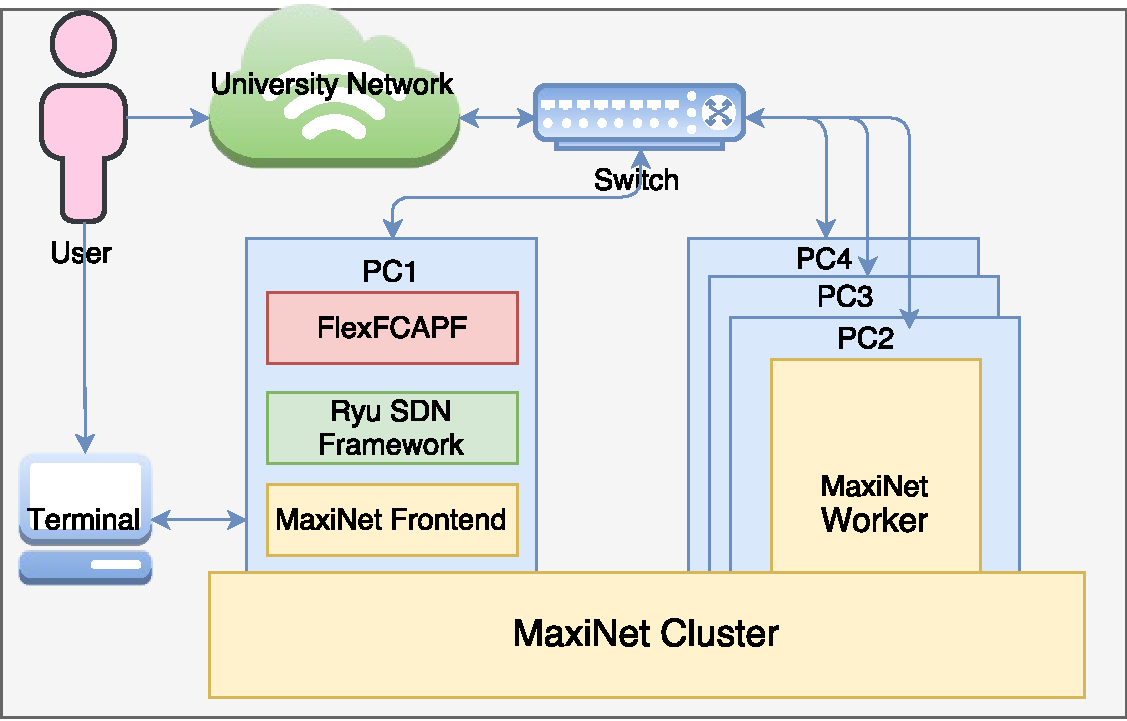
\includegraphics{testbed-infrastructure.pdf}}
		\caption{Overview of testbed infrastructure.}
		\label{fig:testinfra}
	\end{center}
\end{figure}

After selecting the tools and technology, I have to prepare a laboratory setup design, i.e., where to place which components. Figure \ref{fig:testinfra} depicts the overview of the current testbed infrastructure. The testbed consists of four physical machines (PC1, PC2, PC3, and PC4). All four machines are connected to Paderborn University's network with an ethernet switch (20Gbits) using their internal Network Interface Cards (NICs). A terminal is connected to the first machine. A user can access the testbed using the terminal or by using ssh via the university network. PC1 is used as MaxiNet frontend and the other three machines are used as MaxiNet workers. FlexFCAPF and Ryu SDN Framework also run on PC1. These machines altogether build the MaxiNet Cluster.

Before I describe the detailed implementation, it is important to understand the emulation's functional overview, its components, and how they communicate with each other. Figure \ref{fig:testcomp} shows the components of the emulation and how they work together. The emulation is logically divided into four functional modules in high level as follows:
\begin{enumerate}
\item External Module - the Topology Generator and the DFG Generator components fall in this module. Topology Generator communicates with the emulation through input file sharing (topology description). DFG Generator is part of the emulation execution process; it creates DFG dynamically based on some defined parameter (load level, scale). The emulation execution then inserts the DFG into the testbed for further processing.
\item SDN Controller Module - the Ryu SDN controller application is a component of this module and the implementation of a customized SDN controller to match the specific requirement of the emulation is also done under this functional module. The SDN controller communicates with the underlying network elements (switch/router) via TCP socket connection and opens up REST API for FlexFCAPF to communicate with it.
\item Emulator Module - the emulation framework (MaxiNet or Mininet) comes under this module; the network elements (switch/router, host, and links) creation are also implemented under this functional module. Each switch/router is connected to a host, via a link (basically veth pair), and each host running a shell to execute a command on it. Each host has a pipe connected to the emulation framework's parent process (i.e., an instance of the network emulator).
\item FlexFCAPF Module - FlexFCAPF algorithm is implemented as part of this module. The complete FlexFCAPF algorithm is implemented in a class named \textit{CPFlex}. The network emulation instance is a member of the CPFlex class; that way, the CPFlex class instance has direct access to the network. Real traffic generation and data flow processing are also implemented as part of this module.
\end{enumerate}

\begin{figure}[H]
	\begin{center}
		\resizebox{\textwidth}{!}
		{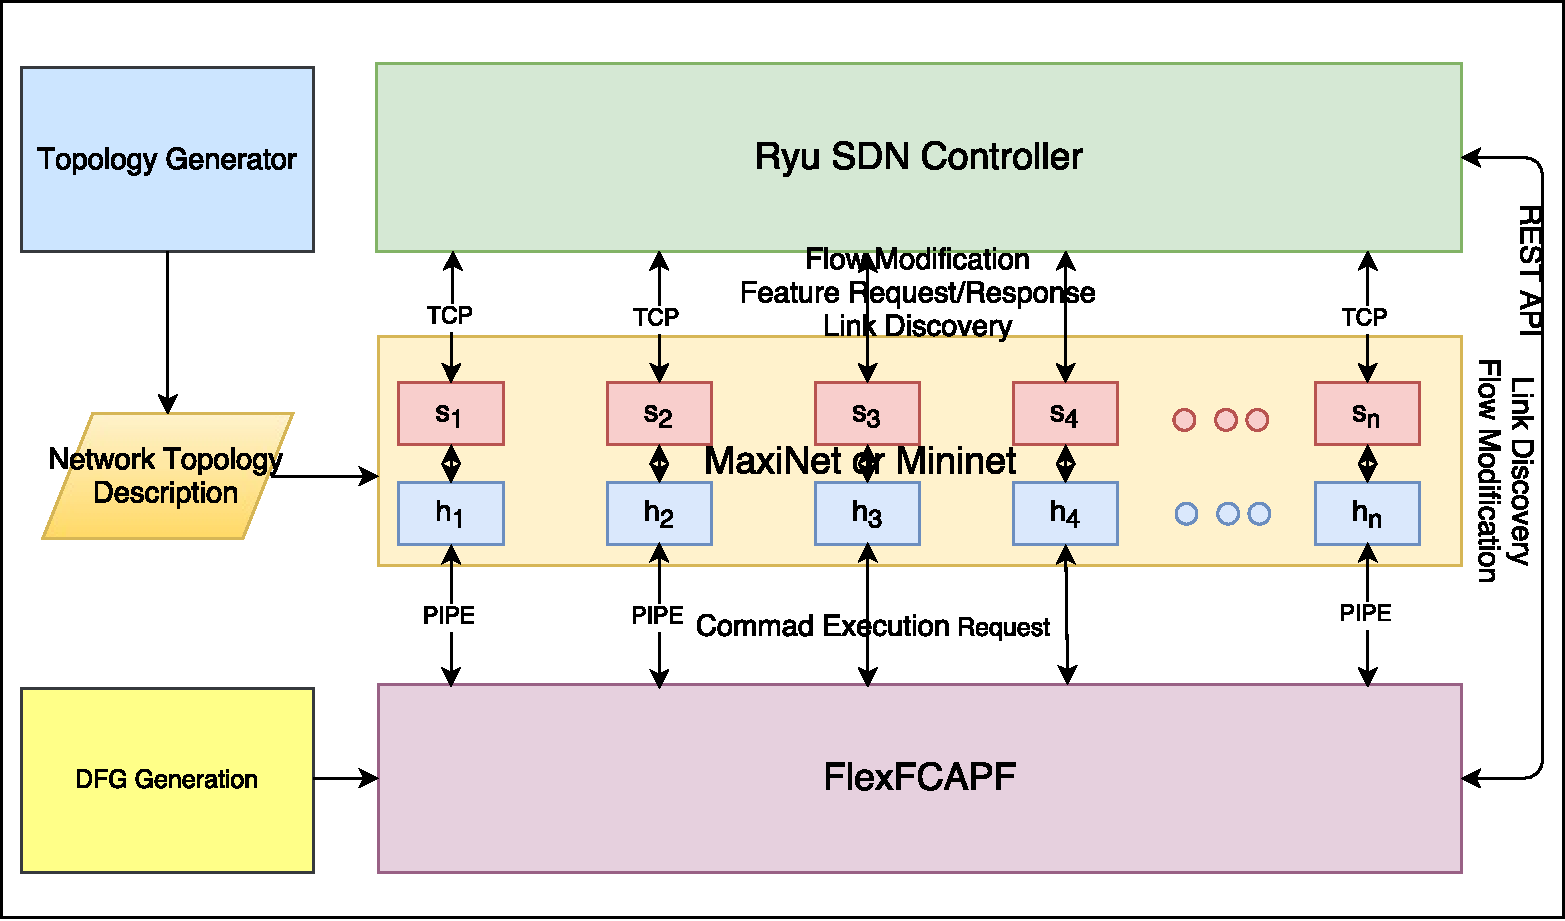
\includegraphics{testbed-components.pdf}}
		\caption{Overview of testbed components.}
		\label{fig:testcomp}
	\end{center}
\end{figure}

The implementation of all the components of each module is discussed in the following sections.

\section{External Module}\label{sec:el}
The emulation needs a topology description to create its underlying network testbed. The topology description is basically the arrangement of network elements of the testbed, e.g., nodes, edge. I am using a python script provided by my supervisor to generate topology description file. It can generate two types of topology, i.e., Mesh and Ring.

Emulation uses similar traffic generation model like the simulation, mentioned in \cite{7343600}. 

The simulation uses a non-stationary Poisson process with $\lambda = |V| \times loadlevel(t)$ and implemented using the thinning method \cite{Law:1999:SMA:554952} for DFG generation. While generating traffic, a daily load level curve (see Figure \ref{fig:24loadlevel}) is followed based on the cellular data traffic characteristics explained in \cite{Zhang:2012:UCC:2342468.2342472}. In emulation, the same model for traffic generation is used with a modified $\lambda = |V| \times loadlevel(t, scaling)$. Load level factor $scaling$ is used to set the scaling of the load level due to the hardware resource limitation in the testbed environment.

\begin{figure}[H]
	\begin{center}
%		\resizebox{\textwidth}{!}
		{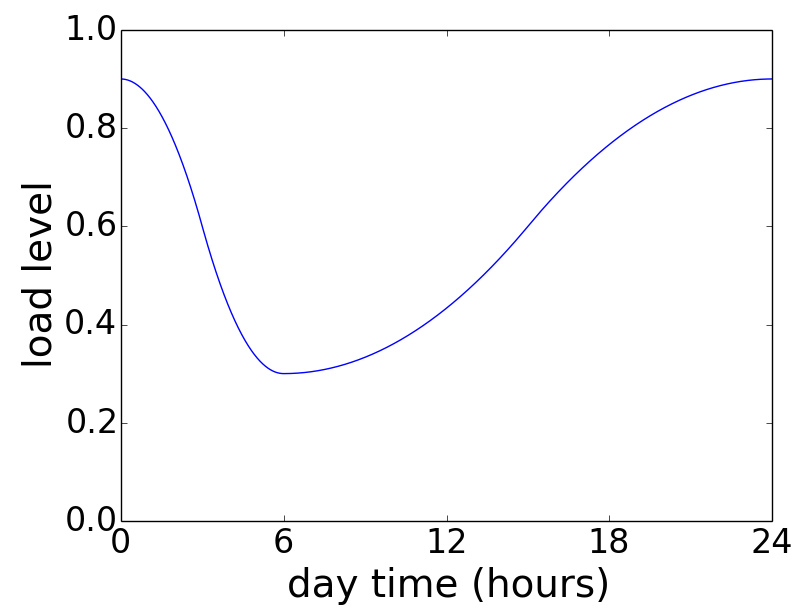
\includegraphics[width=0.40\textwidth]{24-loadlevel.png}}
		\caption{Daily load curve \cite{7343600}.}
		\label{fig:24loadlevel}
	\end{center}
\end{figure}

\section{SDN Controller Module}\label{sec:fca}
Ryu SDN Controller is the component of this module which I developed as part of this study. The SDN controller has mainly two jobs to fulfill, i.e., provide underlying network link details to FlexFCAPF whenever it requests and modifies the forwarding entries in the network elements the way FlexFCAPF wants.

\paragraph{REST Interface Implementation:}
The SDN controller provides a REST interface for serving the request of FlexFCAPF. The Ryu framework has a web server function corresponding to the Web Server Gateway Interface (WSGI). It specifies how a web server can communicate with a web application, and how web applications can be tied together to process one request \cite{wsgi}. By using this functionality, it is possible to create a REST API \cite{ryu}. Ryu has a component \textit{ryu.app.wsgi} which implements that functionality to create REST API.


\begin{lstlisting}[caption={REST API implementation},label={lst:rai},language=Python,tabsize=2,basicstyle=\footnotesize,breaklines=true, showspaces=false,showstringspaces=false,showtabs=false,frame=single]
class ControllerRequestProcessor(ControllerBase)
	def __init__(self, req, link, data, **config):
		super(ControllerRequestProcessor, self).__init__(req, link, data, **config)
		self.fcapf_network_controller = data[fcapp_controller_instance]
	@route('fcapfnetworkcontroller', '/fcapfnetworkcontroller/topology/links', methods=['GET'])
	def list_links(self, req, **kwargs):
		return self._links(req, **kwargs)
\end{lstlisting}

Listing \ref{lst:rai} shows how I implemented REST API in testbed SDN controller. The testbed SDN controller has a class \textit{ControllerRequestProcessor}, it accepts HTTP requests to be processed by Ryu REST AP and is a subclass of \textit{ryu.app.wsgi.ControllerBase}. This way, FlexFCAPF may send the HTTP request to the SDN controller to avail the facility provided by REST API. First, the method \textit{list\_links} is associated with a URL so that the method can be called by HTTP request. It is implemented by a decorator \textit{route} defined in Ryu. The content specified by the decorator have three arguments; the first argument is any name, the second argument is to specify the URL, and the third argument is to specify the HTTP method (e.g., PUT, GET).

\paragraph{Link Discovery Implementation:}
Ryu uses an SDN mechanism called OFDP (OpenFlow Discovery Protocol) to support topology discovery in the network \cite{ofdp}. OFDP internally uses the Link Layer Discovery Protocol (LLDP) \cite{5251812} with slight modifications to perform topology discovery in an OpenFlow network. LLDP allows a network station to advertise their capabilities to other neighbor's station. Ryu has a component called \textit{ryu.topology.api} which is basically the switch and link discovery module of Ryu. I used that module in the testbed SDN controller to retrieve the link details of the network and prepare JSON formatted string and send it to the requesting FlexFCAPF (see Listing \ref{lst:ldr}).

\begin{lstlisting}[caption={Link discovry request},label={lst:ldr},language=Python,tabsize=2,basicstyle=\footnotesize,breaklines=true, showspaces=false,showstringspaces=false,showtabs=false,frame=single]
def _links(self, req, **kwargs):
	dpid = dpid_lib.str_to_dpid(kwargs['dpid'])
	links = get_link(self.fcapf_network_controller, dpid)
	body = json.dumps([link.to_dict() for link in links])
	return Response(content_type='application/json', body=body)
\end{lstlisting}

\paragraph{Event Handler Implementation:}
Once a connection is established between the OpenFlow switch and an SDN controller, the controller can then configure and manage the switch (see Section \ref{par:ofc}). It receives events from the switch and sends packets out to the switch. These handshake procedures are taken care by the Ryu framework itself. The controller usually sends a features request message to know the capabilities of the switch and the switch responds with a features reply message. This is commonly performed upon establishment of the OpenFlow channel \cite{ryubook}. For that purpose, the controller has to save the connection information to access the switch. In Ryu, when an OpenFlow message is received, an event corresponding to the message is generated. I implemented an event handler in the controller corresponding to the desired message to be received as shown in Listing \ref{lst:ehi}. Upon receiving the Switch Features (i.e., features reply from the switch) message in the controller, the \textit{Datapath} object is retrieved and saved for future reference along with the DPID. The \textit{Datapath} class is mainly responsible for actual communication with the OpenFlow switch.


\begin{lstlisting}[caption={Event handler implementation},label={lst:ehi},language=Python,tabsize=2,basicstyle=\footnotesize,breaklines=true, showspaces=false,showstringspaces=false,showtabs=false,frame=single]
class FCAPFNetworkController(app_manager.RyuApp):
	@set_ev_cls(ofp_event.EventOFPSwitchFeatures, CONFIG_DISPATCHER)
	def switch_features_handler(self, ev):
		datapath = ev.msg.datapath
		self.switches[datapath.id] = datapath
\end{lstlisting}

\paragraph{Flow Modification Implementation:}
Upon receiving the request for flow modification (add/delete) request from FlexFCAPF, the SDN controller loop through all entries and modify the flow table in the switch. Initially, I implemented the controller wrongly, i.e., it used to receive one entry per request, but that strategy have a huge performance impact. This is because for each flow modification, FlexFCAPF has to establish an HTTP connection, send the request to the controller, and wait for the response. For a big network, FlexFCAPF has to modify hundreds of flow entries in the network every time a reconfiguration happens. Thus, I changed the logic to process bulk flow modification entries in the controller so that FlexFCAPF can send all flow addition entries in one request and all flow deletion entries in another request. This way, performance improved a lot.

Listing \ref{lst:paei} shows how I implemented the forwarding entry addition in the flow table of a switch. This part of code first converts the datapath id string to a 16-digit hex value defined by \textit{DPID\_PATTERN} of Ryu library. It uses the \textit{FCAPFNetworkController} instance to retrieve the datapath object matching the hex DPID. It is important to remember that the DPID and the datapath object mapping were saved during the features message handling. The input flow configuration entry is parsed and converted to the Ryu supported format. The controller uses action type \textit{ofproto\_v1\_3.OFPP\_NORMAL}, which means the packet will be forwarded by the L2/L3 switch function. A match object is generated calling the constructor of \textit{OFPMatchto} class based on the ethernet frame type (e.g., IP, ARP). Finally, priority 1 is set and the \textit{\_add\_flow} method is called to sent the Flow Mod message.

\begin{lstlisting}[caption={Processing add entry implementation},label={lst:paei},language=Python,tabsize=2,basicstyle=\footnotesize,breaklines=true, showspaces=false,showstringspaces=false,showtabs=false,frame=single]
def _set_flow_table(self, dpid_str, entry):
	dpid = dpid_lib.str_to_dpid(dpid_str)
	contr_inst = self.fcapf_network_controller
	datapath = contr_inst.switches.get(dpid)
	if action == 'normal':
		action = ofproto_v1_3.OFPP_NORMAL
	if datapath is not None:
		parser = datapath.ofproto_parser
		actions = [parser.OFPActionOutput(action)]
		if dl_type == "ip":
			port = entry['inport']
			match = parser.OFPMatch(in_port=port, ipv4_src=ip_src,ipv4_dst=ip_dest, eth_type=0x0800)
		elif dl_type == "arp":
			match = parser.OFPMatch(arp_spa=ip_src, arp_tpa=ip_dest, eth_type=0x0806)
		else:
			LOG.error("Wrong input!!")
		self._add_flow(datapath, 1, match, actions)
\end{lstlisting}

The processing of the forward entry addition is not done yet. The method \textit{\_add\_flow} set the instruction to use the \textit{ofproto.OFPIT\_APPLY\_ACTIONS} so that the specified action is immediately used. I created a class instance of \textit{OFPFlowMod} to prepare the modification message and the message is sent to the OpenFlow switch using the method \textit{datapath.send\_msg} call to add the forwarding entry in the flow table (see Listing \ref{lst:afei}).
\begin{lstlisting}[caption={Add forwarding entry implementation},label={lst:afei},language=Python,tabsize=2,basicstyle=\footnotesize,breaklines=true, showspaces=false,showstringspaces=false,showtabs=false,frame=single]
def _add_flow(self, datapath, priority, match, actions, buffer_id=None):
	parser = datapath.ofproto_parser
	inst = [parser.OFPInstructionActions(datapath.ofproto.OFPIT_APPLY_ACTIONS, actions)]
	mod = parser.OFPFlowMod(datapath=datapath, priority=priority, match=match, instructions=inst)
	datapath.send_msg(mod)
\end{lstlisting}
The deletion of forwarding entry from the flow table is similar to addition, therefore the description of that code which does the processing of deletion entry request is not presented. The difference is, while preparing forwarding entry modification message, here, a command \textit{ofproto.OFPFC\_DELETE} is used to specify the action of deleting forwarding entry while creating \textit{OFPFlowMod} class instance (see Listing \ref{lst:dfei}).
\begin{lstlisting}[caption={Delete forwarding entry implementation},label={lst:dfei},language=Python,tabsize=2,basicstyle=\footnotesize,breaklines=true, showspaces=false,showstringspaces=false,showtabs=false,frame=single]
def _del_flow(self, datapath, match):
	ofproto = datapath.ofproto
	parser = datapath.ofproto_parser
	mod = parser.OFPFlowMod(datapath, command=ofproto.OFPFC_DELETE, out_port=ofproto.OFPP_ANY, out_group=ofproto.OFPG_ANY,priority=1, match=match)
	datapath.send_msg(mod)
\end{lstlisting}

\section{Emulator Module}\label{sec:emmod}
The underlying network is the component of this module; the network can be created either using the MaxiNet or Mininet emulation framework. I started to implement the testbed with a small number of nodes using Mininet and tried prototyping experiments in Mininet. Later, I introduced MaxiNet in code and implement the whole process in a flexible manner. Since MaxiNet is based on Mininet, it was easy to keep both options available. One can choose either Mininet or MaxiNet while starting the experiment. The testbed network is created based on the user provided topology description files (see Section \ref{sec:el}). The \textit{CPFlex} instance takes the topology description file as input and converts it to an in-memory graph to represent the structure of the network using a user defined python class \textit{CrowdNetwork}. \textit{CrowdNetwork} internally uses the python package \textit{NetworkX} for storing the testbed structure in memory which I call FlexFCAPF network model. \textit{CrowdNetwork} class was developed by my supervisor as part of a simulation work. Network creation steps are similar for both MaxiNet and Mininet; only some API's are different. Here, I describe the common as well as the different network creation steps.

\subsection{Setup Network}\label{sec:setnet}
Listing \ref{lst:sni} shows how I set up the network using Mininet or MaxiNet. Both creates a \textit{Topo} object, a flexible empty topology (topo) with two parameters, \textit{TCLink} and \textit{CPULimitedHost}. \textit{TCLink} and \textit{CPULimitedHost} classes provide the option of setting limitation on link bandwidth, delay, loss, and host processing power. A standard naming convention for the host ($h_0 ... h_n$) and switch($s_0 ... s_n$) is followed. The standard is followed while assigning unique IP, MAC (to hosts), DPID, and listen port (to switches) as well. This standardization would help us track the hosts and switches. A node in FlexFCAPF model is represented by a host and a switch combination in the network. Switches are running in kernel level to get a better speed of communication between multiple hops in the network (see Section \ref{sec:mininet}). A host is attached to each switch to run some user-level process (e.g., flow generation). A link is added between the switch and its associated host and links are added for all the edges specified in FlexFCAPF model.
\begin{lstlisting}[caption={Setup network implementation},label={lst:sni},language=Python,tabsize=2,basicstyle=\footnotesize,breaklines=true, showspaces=false,showstringspaces=false,showtabs=false,frame=single]
def setupEmulationNetwork(self):
	topo = Topo(link=TCLink, host=CPULimitedHost)
	linkopts = dict()
	# Add switches and associated hosts
	s = 1
	for n in self.cn.G.node:
		hName = 'h' + str(n)
		hIp = Tools.makeIP(n + 1)
		hMac = Tools.makeMAC(n + 1)
		hObj = topo.addHost(name=hName, ip=hIp, mac=hMac)
		self.Hosts[hName] = {'obj': hObj, 'ip': hIp, 'mac': hMac}
		sName = 's' + str(n)
		sDpid = Tools.makeDPID(n + 1)
		sListenPort = (13000 + s - 1)
		switchopts = dict(listenPort=sListenPort)
		sObj = topo.addSwitch(name=sName, dpid=sDpid, **switchopts)
		self.Switches[sName] = {'obj': sObj, 'dpid': sDpid, 'listenport': sListenPort}
		s += 1
		topo.addLink(hObj, sObj, **linkopts)
	for key, value in self.cn.G.edges():
		sName1 = 's' + str(key)
		sName2 = 's' + str(value)
		sObj1 = self.Switches[sName1]['obj']
		sObj2 = self.Switches[sName2]['obj']
		topo.addLink(sObj1, sObj2, **linkopts)
\end{lstlisting}

\paragraph{Starting Network:}
This step is different for MaxiNet and Mininet since nodes are distributed across multiple physical machines in MaxiNet. MaxiNet first creates a cluster object and then pass the topo object along with the cluster object and switch parameter to create an \textit{Experiment} object. Finally, call the \textit{setup()} method using the experiment object to start the emulation. Whereas Mininet creates a Mininet object using the \textit{Topo} object, switch parameter and controller parameter and start the emulation network by calling the \textit{start()} method. The OpenFlow protocol version 1.3 is passed while creating Mininet network and the same is done for MaxiNet as well in a later step. Controller parameter with a value of \textit{RemoteController} is used so that the SDN controller may run anywhere on the network, but which must be started up and shut down manually or by some other mechanism outside of Mininet's direct control. MaxiNet by default run the controller with that option because MaxiNet internally starts multiple instances of Mininet and runs in a distributed environment. The Mininet network object or MaxiNet Experiment object is saved in a member variable of \textit{CPFlex} class for future reference. 

Listing \ref{lst:stni} shows the code implementation of the same.
 
\begin{lstlisting}[caption={Starting network implementation},label={lst:stni},language=Python,tabsize=2,basicstyle=\footnotesize,breaklines=true, showspaces=false,showstringspaces=false,showtabs=false,frame=single]
if self.emulator == "Mininet":
	# Mininet
	switch = functools.partial(OVSSwitch, protocols='OpenFlow13')
	net = Mininet(topo=topo, switch=switch, controller=RemoteController, host=CPULimitedHost, link=TCLink)
	net.start()
	# Save the Mininet object for future reference
	self.TestbedNetwork = net
elif self.emulator == "MaxiNet":
	# MaxiNet
	cluster = maxinet.Cluster()
	exp = maxinet.Experiment(cluster, topo, switch=OVSSwitch)
	exp.setup()
	# Save the Experiment object for future reference
	for switch in exp.switches:
		exp.get_worker(switch).run_cmd('ovs-vsctl -- set Bridge %s ' % switch.name + 'protocols=OpenFlow10,OpenFlow12,OpenFlow13')
	self.TestbedNetwork = exp
else:
	exit(1)
\end{lstlisting}

\paragraph{Running User Process:}
One important requirement of the emulation is to emulate a way to achieve data processing capability in the network. To achieve that functionality, a user process needs to be run in the Mininet/MaxiNet host, which is assigned as an LCA. The job of that process is to work as a packet receiver or sink and resend the received packet back to the source. Each Mininet/MaxiNet host is essentially a bash shell process attached to one or more network interfaces, so the easiest way to interact with it is to send input to the shell using the \textit{cmd()} method. I used that facility to run \textit{socat} listener process in each potential LCA host to receive the flow in the LCA. A \textit{/bin/cat} is executed by the \textit{socat} to resend the packet back to the source. Listing \ref{lst:rupi} shows the code implementation for the same.

\begin{lstlisting}[caption={Running user process implementation},label={lst:rupi},language=Python,tabsize=2,basicstyle=\footnotesize,breaklines=true, showspaces=false,showstringspaces=false,showtabs=false,frame=single]
for n in self.cn.G.node:
	if n in self.cn.C:
		hName = 'h' + str(n)
		hObj = self.TestbedNetwork.get(hName) if self.emulator == "Mininet" else self.TestbedNetwork.get_node(hName)
		hObj.cmd("socat -T 5 UDP-LISTEN:5001,fork,reuseaddr EXEC:\'/bin/cat\' &")
\end{lstlisting}

Here, the socat instance running on the LCA host acts as receiver of the packet as well as the generator of the duplicate packet to resend. The socat server instance keeps listening to port 5001 (the default port for iperf connection) continuously and waits for the client connection. When a client connection request comes in, the socat starts a child process to serve that client. One important point to notice here is the parameter \textit{-T} for specifying inactivity timeout. Initially, I was not using it and due to that, there were many child processes that keep running for hours even though the client (iperf) from the other end stopped sending packets. This ate up a lot of system resources and slowed down the complete processing. Introducing this timeout solve that problem. When socat is already in the data receiving loop and nothing has happened (no data arrived, no interruption occurred) for the timeout seconds, then the serving child process terminates. But the parent socat process stays alive to accept connection. Since I am using UDP traffic, this functionality is very useful for terminating the remote server as UDP cannot transfer EOF (see Section \ref{sec:tragen}).

\section{FlexFCAPF Module}
The components of this module are FlexFCAPF algorithm, routing table modification, traffic flow generation, and data flow processing (partially). FlexFCAPF algorithm was implemented as part of simulation evaluation, therefore, I will skip the detailed code-level description. However, it is important to know how the algorithm works to understand the complete emulation so I give an overview of the algorithm.

\subsection{FlexFCAPF Algorithm} \label{sec:algoadap}
In this section, I describe how FlexFCAPP algorithm works. Functionality wise, the complete algorithm has two parts. First is the initial controller placement functionality of FlexFCAPF, and second, the flexible reassignment functionality. To provide an initial overview, Figure \ref{fig:flexfcpfflow} outlines the key aspects of FlexFCAPF in a flow chart. This algorithm description is prepared based on the implementation of the algorithm specified in \cite{7343600}.

\begin{figure}[H]
\begin{center}
	\resizebox{\textwidth}{!}
	{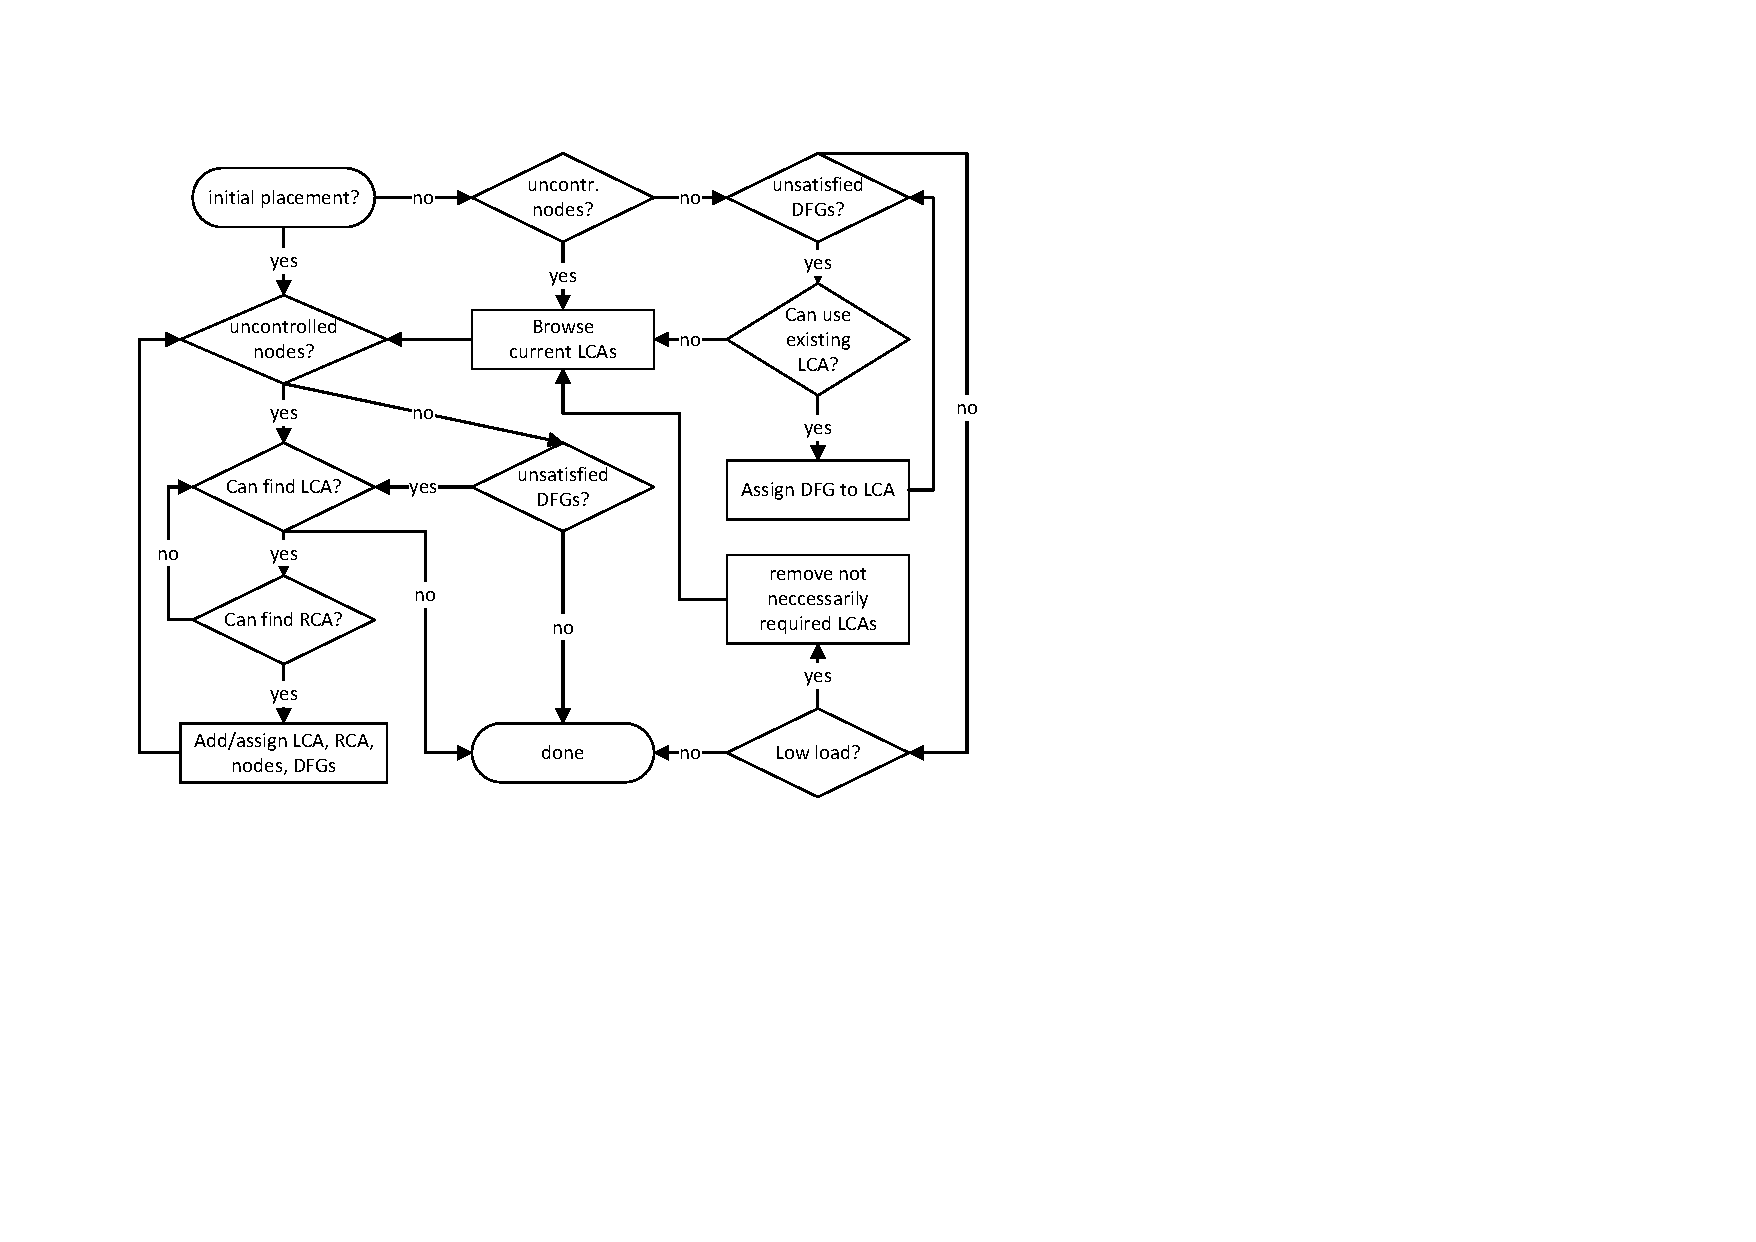
\includegraphics{flexfcpf-flowchart.pdf}}
	\caption{FlexFCAPF flow chart \cite{7343600}.}
	\label{fig:flexfcpfflow}
\end{center}
\end{figure}

\paragraph{Initial Controller Placement:}
FlexFCAPF works on a valid network; it is an internal state to specify that a network model is generated from an input topology description file successfully without any exception (see Section \ref{sec:emmod}). The algorithm first focus on node control, i.e., assign at least one LCA to each node of the network, then it changes focus to DFG satisfaction. The algorithm ends its execution if all DFGs are satisfied, if no more CAs are available, or if no new DFGs could be satisfied by adding an additional LCA, e.g., if all remaining DFGs cannot be satisfied with the network's remaining resources. At the end, the algorithm may clean up all LCA-to-node assignments that eventually did not serve any purpose, i.e., the LCA does not satisfy any data flow passing through the node and the node is assigned to more than one LCA.

To assign an LCA to a node, the algorithm has to determine the next potential CA to be added as LCA and get the appropriate LCA candidate based on different criteria. Then it makes sure an RCA is assigned to the selected candidate before adding it as LCA. This step is necessary to maintain the integrity of the two-layer CAs architecture (see Section \ref{sec:fcpf}). The candidate is confirmed as a new LCA if an RCA is found for it and can be assigned to the RCA.

To assign RCA to an LCA, the algorithm first try to get the nearest available RCA from the available RCAs. If no existing RCA can be assigned to an LCA candidate, a new RCA is added to the network considering all potential CAs that are not yet RCAs. FlexFCAPF tries to look for the most centralized potential RCA while looking for the first RCA in order to benefit all future RCA-to-LCA assignments. Otherwise, FlexFCAPF goes by the distance from RCA to the requesting LCA candidate. 

Once a node is assigned as an LCA, the algorithm also tries to assign DFGs to the new LCA ($v$). Depending on whether a network already has a complete control structure or not, it calculates the shortest paths from $v$ to all other nodes in the network. Later, the nodes are assigned to be controlled by the new LCA ($v$). During this process, the algorithm verifies that no model constraint is violated (see Section \ref{sec:ffps}).

When a node is assigned to LCA $v$, the algorithm updates the list of potential DFGs for $v$, i.e., the DFGs that are only passing through nodes that $v$ already controls and thus can be satisfied by $v$, provided there is sufficient resources available. Moreover, when $v$ is allowed to satisfy DFGs, FlexFCAPF successively try to assign the most demanding (in terms of requested processing capacity) DFG to $v$. The algorithm check all constraints before confirming a certain DFG is satisfied by $v$ (see Section \ref{sec:ffps}). In any case, the DFG is removed from the list of potential DFGs for $ v$, as it is either now satisfied by $v$ or it cannot be satisfied by $v$. 

Also, FlexFCAPF introduces a constraint, i.e., DFGs may only be satisfied by an LCA once it controls at least \textit{VCRatio} nodes that have previously been uncontrolled or if there are no more uncontrolled nodes in the network. Consider a situation where a network has many DFGs, and hence each LCA would have a lot of potential DFGs. After controlling only a few nodes, the LCAs may run out of resources by quickly satisfying many DFGs. In that case, a complete control structure would probably not be obtained. Hence, FlexFCAPF introduced that constraint to deal with such situation. At starting, VCRatio is initialized with a value $VCRatio = \frac{|V|}{|C|}$. 

\paragraph{Flexible Reassignment:}
There could be two scenarios which would trigger the network configuration change, i.e., reassignment of LCAs. One is Incoming DFGs and another is Low Load Situations. When a new DFG is added in the network, FlexFCAPF tries to assign it to one of the existing LCAs in the network. It first tries to assign the incoming DFG to the nearest possible LCA. If it fails to satisfy an incoming DFG, FlexFCAPF normally add a new LCA in the network and that will satisfy the new DFG.

Identifying a Low Load Situation is easy, but it is not trivial to remove an LCA while still satisfying all the DFGs in the network. FlexFCAPF continuously monitors the average LCA load in the network and if it stays below a threshold value, i.e., LCAloadlimit = 0.9 for 10 seconds or more, it removes unnecessary LCAs. This step will eventually move all the nodes and DFGs currently satisfied by the removed LCA to unsatisfied state again. Then, FlexFCAPF tries to assign those nodes and DFGs among all available LCAs. If FlexFCAPF could not reduce the number of LCAs from its earlier number, then, the low load correction is considered as failed and the LCAloadlimit is decreased by 0.05 for the next round.

\subsection{Modify Routing Table}\label{sec:mrt}
This is an important step for emulation. In emulation, real traffic is generated and that traffic has to follow a defined path (traffic generating node to its satisfying LCA) specified by FlexFCAPF algorithm. Every time FlexFCAPF algorithm is executed, there might be some new LCA introduced or may be some LCA removed. That would cause some nodes to be reassigned to new LCAs; this way, the path between the nodes and LCAs might change. To be in sync with the algorithm execution results, the emulation needs to modify the routing entries in the underlying network. The whole process is divided into three steps, i.e., populate network links, add routing entries, and delete routing entries.

\paragraph{Populate Network Links:}
The population of network links is a one-time job and this is done after starting the emulation network. Once the virtual network is created, all the connection between the network elements is retrieved by the Ryu SDN controller and saved it in an in-memory structure. This includes all the links' details and the interfaces belonging to each link. This is done by calling REST API provided by the controller over HTTP request. This information is necessary because the routing entries in the underlying network have to be in sync with FlexFCAPF defined path. That is why the emulation prepares each forwarding entry which needs to be added in the underlying network elements. The emulation uses this information while preparing the forwarding entries for the underlying network. Listing \ref{lst:pnli} shows the code implementation of the same.

\begin{lstlisting}[caption={Populate network links implementation},label={lst:pnli},language=Python,tabsize=2,basicstyle=\footnotesize,breaklines=true, showspaces=false,showstringspaces=false,showtabs=false,frame=single]
def populateNetworkLinks(self):
	urlpath = "http://127.0.0.1:8080/fcapfnetworkcontroller/topology/links"
	resp = requests.get(urlpath)
	self.Links = resp.json()
\end{lstlisting}

\paragraph{Add Routing Entries:}
This step has to be executed every time FlexFCAPF algorithm is executed. The method \textit{modifyRoutingTable} (see Listing \ref{lst:mrti}) is responsible for that purpose. When this method is called for the first time, it loops through all the path between the nodes and it satisfies the LCA. It prepares an entry request for each link in the path by calling the method \textit{addRoutingPath}. Before that, it checks if the routing path between them already exists or not by calling \textit{checkRoutingPath} method.

\begin{lstlisting}[caption={Modify routing table implementation},label={lst:mrti},language=Python,tabsize=2,basicstyle=\footnotesize,breaklines=true, showspaces=false,showstringspaces=false,showtabs=false,frame=single]
def modifyRoutingTable(self):
	for n in self.cn.G.node:
		node = self.cn.G.node[n]
		pathToLCA = node['pathtoLCA']
		for clc, path in pathToLCA.items():
			src = clc
			dst = n
			foundPath = self.checkRoutingPath(src, dst, path)
			if foundPath == False:
				self.addRoutingPath(src, dst, path)
	self.requestAddRoutingEntries()
	self.clearObsoleteRoutingPaths()
	self.requestDeleteRoutingEntries()
\end{lstlisting}
The \textit{checkRoutingPath} (see Listing \ref{lst:crpi}) checks it by comparing the input path with its earlier saved list of the path in an in-memory structure \textit{RoutingPaths}. If the path is not present in the in-memory structure \textit{RoutingPaths}, it adds the path in that structure. It also prepares a temporary list of all current paths \textit{CurrentRoutingPaths}. By adding the non-existing path in the network, the emulation gets two benefits. First, it is only adding the difference path but not the complete path, thus, saving processing time for the controller and the underlying network elements. Another benefit is, it is not disturbing the traffic which is running in the network at that moment.

\begin{lstlisting}[caption={Check routing path implementation},label={lst:crpi},language=Python,tabsize=2,basicstyle=\footnotesize,breaklines=true, showspaces=false,showstringspaces=false,showtabs=false,frame=single]
def checkRoutingPath(self, src, dst, path):
	key = (src, dst, path)
	self.CurrentRoutingPaths.append(key)
	foundPath = key in self.RoutingPaths
	if foundPath == False:
		self.RoutingPaths.append(key)
	return foundPath
\end{lstlisting}

The \textit{addRoutingPath} method prepares the flow table entry information with the help of the real links information which is saved earlier and add those entries to a list \textit{JsonEntries} for creating forwarding entry in the network. For each link in a path, a total of four entries will be created, i.e., one for inward traffic and one for outward traffic; and for each way traffic, two types of entries is created, one for ARP packet and another for IP packet. Since it is a lengthy repetitive code, the code implementation is not presented here for this method. One important point to remember is that a standard was followed for assigning the IP address to host and MAC address to the switch while creating the network. That information is necessary to create the forwarding entries in the network elements. Because the forwarding entry's match conditions are prepared based on the source IP address, destination IP address and the MAC address are necessary for specifying where to add the entry.

The \textit{requestAddRoutingEntries} (see Listing \ref{lst:rarei}) method takes all the \textit{JsonEntries}, the newly prepared flow table entry list, and calls the \textit{addflows} REST API provided by the controller to actually create forwarding rules in the underlying network elements.
\begin{lstlisting}[caption={Request add routing entries implementation},label={lst:rarei},language=Python,tabsize=2,basicstyle=\footnotesize,breaklines=true, showspaces=false,showstringspaces=false,showtabs=false,frame=single]
def requestAddRoutingEntries(self):
	url = "http://127.0.0.1:8080/fcapfnetworkcontroller/flowtable/addflows"
	data = json.dumps(self.JsonEntries)
	resp = requests.put(url, data=data)
	if resp.status_code != 200:
		print "Something is wrong adding Routing entries, check controller log!!"
	del self.JsonEntries
	self.JsonEntries = []
\end{lstlisting}

\paragraph{Delete Routing Entries:}
Similar to the add routing entries, the delete routing entries also have two steps; first, it cleans up all the obsolete entries from the in-memory routing path, i.e., \textit{RoutingPaths}. The method \textit{clearObsolateRoutingPaths} (see Listing \ref{lst:corei}) is used to clean up all the obsolete paths which are present in the in-memory \textit{RoutingPaths}. This is done by comparing two list of routing paths, i.e., \textit{RoutingPaths} and \textit{CurrentRoutingPaths}. It is important to notice that \textit{CurrentRoutingPaths} is prepared in the method \textit{checkRoutingPath} during add routing entries. The \textit{CurrentRoutingPaths} contains only those entries which are provided by last FlexFCAPF run and \textit{RoutingPaths} contains all the entries which are already added in the underlying network. The path provided by the latest run only should exist in the underlying network, others have to be removed. For doing that, the \textit{clearObsoleteRoutingPaths} calls \textit{deleteRoutingPath} method to prepare a list of \textit{JsonEntries} which needs to be removed from the underlying network. Finally, \textit{requestDeleteRoutingEntries} is used to remove forwarding rules from the network elements. The method \textit{requestDeleteRoutingEntries} acts similarly like \textit{requestAddRoutingEntries}, i.e., calls the \textit{delflows} REST API provided by the controller. The method \textit{deleteRoutingPath} also works similar to \textit{addRoutingPath}.

\begin{lstlisting}[caption={Clear obsolete routing entries implementation},label={lst:corei},language=Python,tabsize=2,basicstyle=\footnotesize,breaklines=true, showspaces=false,showstringspaces=false,showtabs=false,frame=single]
def clearObsoleteRoutingPaths(self):
	entries = copy.deepcopy(self.RoutingPaths)
	for entry in entries:
		(src, dst, path) = entry
		if entry not in self.CurrentRoutingPaths:
			self.deleteRoutingPath(src, dst, path)
			self.RoutingPaths.remove(entry)
	del entries
	del self.CurrentRoutingPaths
	self.CurrentRoutingPaths = []
\end{lstlisting}
It is important to note that the REST API calls are made two times: once for adding and once for deleting flow entries. This is done to reduce parsing efforts at the controller. If the controller receives both types of request at the same time, it has to check each entry for the type of request. By separating addition and deletion in two calls, the logical implementation is also kept separate.

\subsection{DFG Processing}\label{sec:tmfg}
Implementing real data processing is not a feasible option in the emulation environment due to resource constraints, i.e., it needs a hardware with more CPU power and memory. I developed an alternative way achieve data processing capability in the CA. Ideally, there are three steps necessary to have a real data processing in the testbed. These steps are capturing the packet, executing some processing logic on the packet, and sending the packet back to the source. The concept of data processing here is, instead of doing some real processing on the captured packet and resending it back to the source, just delay the packet in the CA before sending. The idea is actual processing (i.e., run some processing logic) would take some time, e.g., $\Delta t$; instead of running processing logic, simply delay the packet in CA for that $\Delta t$ time and then send the packet back to the source. This way, by introducing a waiting time for each packet in the CA, the processing capability is achieved. The waiting time for each packet of different DFG would not be the same; each DFG would need a different processing time, i.e., delay. To deal with this problem, I introduced a concept of adding an identifier to the packet. FlexFCAPF gives processing time (delay) required for processing a packet of a particular DFG. Now, I have the packet identifier and the delay needs to be applied on the packet. Using this information, I am configuring filters and queues in the CAs. This is done using Linux networking tools \textit{tc} and \textit{netem} (see Section \ref{sec:tan}).

\begin{figure}[H]
	\begin{center}
		\resizebox{\textwidth}{!}
		{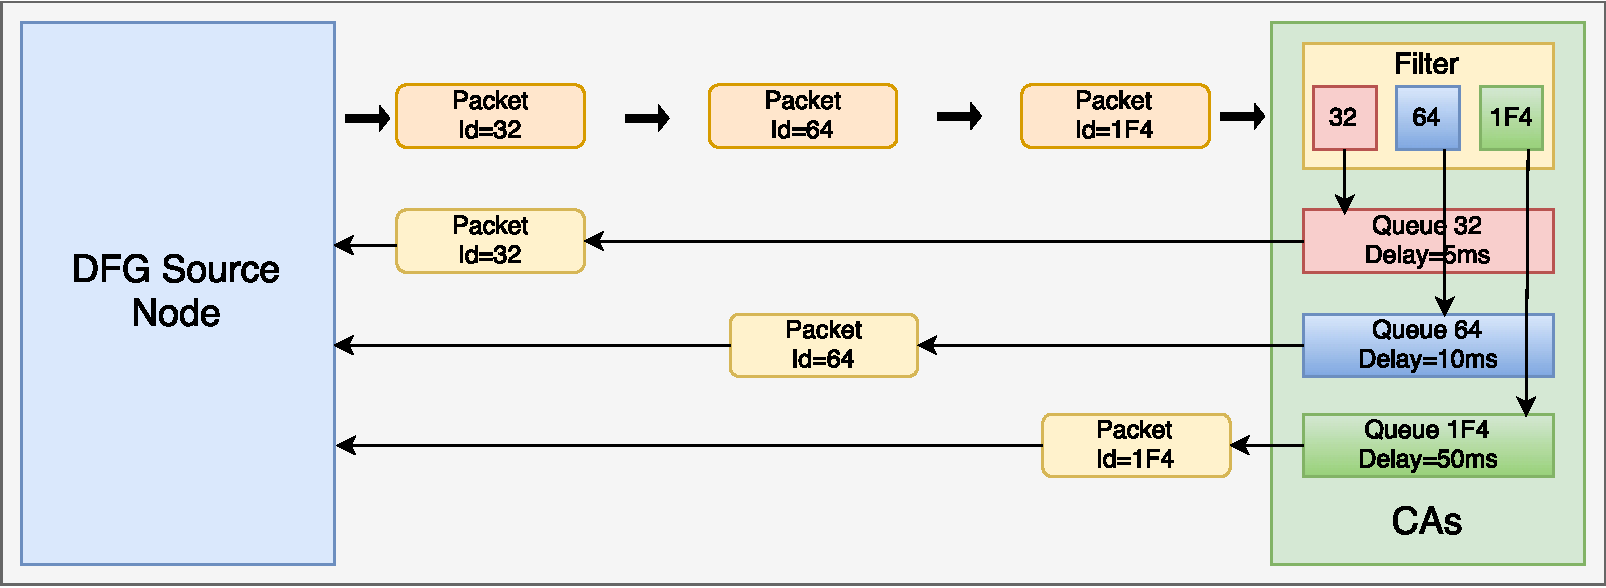
\includegraphics{dataprocessing.pdf}}
		\caption{Data processing overview.}
		\label{fig:dataproc}
	\end{center}
\end{figure}

Figure \ref{fig:dataproc} shows an overview of the data processing implementation in the testbed. The traffic generator in the DFG source node adds an identifier to each packet it generates (see Section \ref{sec:tragen}). Then, the packet travels through the network and reaches the satisfying LCA, and in turn, the LCA sends the same packet back to the source. When the packet goes out of the LCA, the data processing delay is applied on the packet. Before starting traffic generation, a delay configuration needs to be done in the satisfying LCA. The traffic control configuration is done by executing a small script shown in listing \ref{lst:cdi} on the LCA.

\begin{lstlisting}[caption={Configure delay implementation},label={lst:cdi},language=bash,tabsize=2,basicstyle=\footnotesize,breaklines=true, showspaces=false,showstringspaces=false,showtabs=false,frame=single]
if tc qdisc show dev "$interface" | grep "qdisc htb $r_handle:" > /dev/null; then
	qdpresent=true
else
	qdpresent=false
fi
if [ $qdpresent != true ]; then
	if not ( tc qdisc add dev "$interface" root handle $r_handle: htb;) then
		exit 1
	fi
fi
if not (tc class add dev "$interface" parent $r_handle: classid $r_handle:$n_handle htb rate 2500Mbit;) then
	exit 1
fi
if not (tc qdisc add dev "$interface" parent $r_handle:$n_handle handle $n_handle: netem delay ${delay}ms;) then
	exit 1
if not (tc filter add dev "$interface" parent $r_handle:0 protocol ip prio 1 u32 classid 1:$n_handle match u32 $flowid 0xffffffff at 28;) then
	exit 1
fi
\end{lstlisting}

To configure the delay for each specific Id of the packet, three traffic control objects (a \textit{class}, a \textit{qdisc}, and a \textit{filter}) need to be configured in the output network interface of the LCA host. The queue (i.e., \textit{qdisc}) is associated with the \textit{class} and the delay value (which is applied to the outgoing packet) is assigned to the queue, and all these classes are associated to a root queue. The \textit{filter} is directly associated with the root queue and it has an additional association with the class. The \textit{filter} has a match condition and the match condition is set as the packet identifier. Therefore, whenever a packet goes out of the LCA, the \textit{filter} matches the packet data field (the field where the identifier is saved), and if a match is found, that packet will be handled by the respective class associated with the filter. Eventually, the class will put the packet in the queue which is attached to the class. The packet will wait in the queue for the configured delay specified for the queue, then the packet will go out of the LCA after waiting for the delay. It is important to remember here that the LCA will return the same packet back, no modification is done in the packet inside the LCA. So the packet will contain the identifier which is set by the generator. 

Listing \ref{lst:tcoce} shows a sample traffic control object's configuration setup. This is done by the shell script in Listing \ref{lst:cdi}, the script takes five input parameters: the interface, the root key, a child key (usually the packet identifier), the delay and the match condition (this is also the packet identifier but HEX value). First, the script checks for the root qdisc if not present then add the root qdisc in the interface with handle = ``rootkey:". Then it adds a class with classid = ``rootkey:childkey" and a child qdisc with handle = ``childkey:", parent = ``rootkey:childkey" and netem delay = ``delay value" in the interface. Finally, it adds a filter in the interface with parent = ``rootkey:0", classid = ``1:childkey" and match condition = ``match condition value"

\begin{lstlisting}[caption={Traffic Conroller object's configuration example},label={lst:tcoce},language=bash,tabsize=2,basicstyle=\footnotesize,breaklines=true,showspaces=false,showstringspaces=false,showtabs=false,frame=single]
$h10 tc class show dev h10-eth0
class htb 1:100 root leaf 100: prio 0 rate 2500Mbit ceil 2500Mbit burst 1250b cburst 1250b
class htb 1:500 root leaf 500: prio 0 rate 2500Mbit ceil 2500Mbit burst 1250b cburst 1250b

$h10 tc qdisc show dev h10-eth0
qdisc htb 1: root refcnt 2 r2q 10 default 0 direct_packets_stat 17188 direct_qlen 1000
qdisc netem 100: parent 1:100 limit 1000 delay 10.0ms
qdisc netem 500: parent 1:500 limit 1000 delay 50.0ms

$h10 tc filter show dev h10-eth0
filter parent 1: protocol ip pref 1 u32
filter parent 1: protocol ip pref 1 u32 fh 800: ht divisor 1
filter parent 1: protocol ip pref 1 u32 fh 800::800 order 2048 key ht 800 bkt 0 flowid 1:100 match 00000064/ffffffff at 28
filter parent 1: protocol ip pref 1 u32 fh 800::801 order 2049 key ht 800 bkt 0 flowid 1:500 match 000001f4/ffffffff at 28
\end{lstlisting}

Figure \ref{fig:tcobjhier} shows an example of Traffic Control object's hierarchy of a network interface. Each interface has a root queue (qdisc), which is the default. For packet identifier ``00000064", an HTB class with id ``1:100", a netem qdisc with id ``100:", and a filter with id ``800::801" associated to class id ``1:100" are configured. The qdisc with id ``100:" have a delay of 10.0ms and the filter with id ``800::801" have a match condition ``"00000064/ffffffff" configured. This means when a packet with identifier ``00000064" goes out of this interface, it will be delayed by 10.0ms. Similarly, for packet identifier ``000001f4", the same set of objects are configured.

\begin{figure}[H]
	\begin{center}
		\resizebox{\textwidth}{!}
		{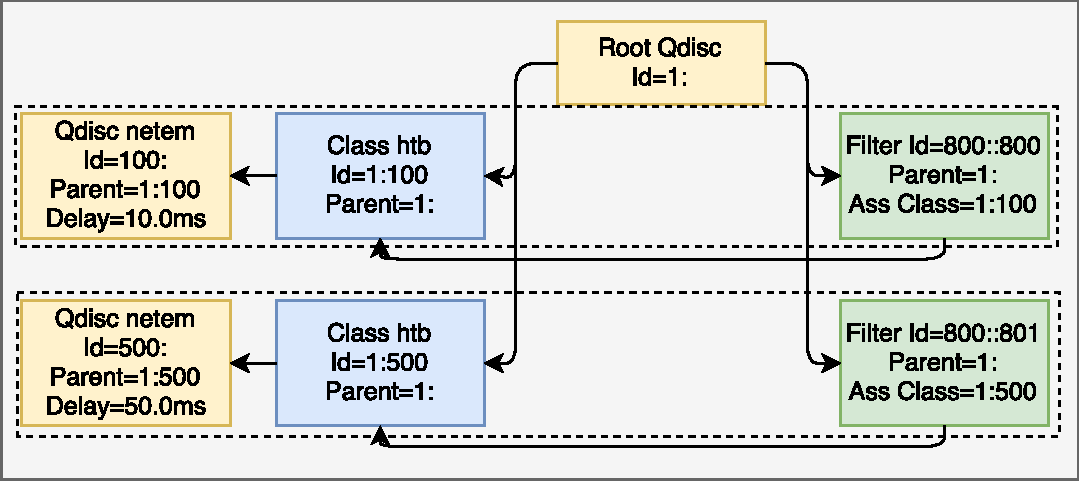
\includegraphics{tcobjectshierarchy.pdf}}
		\caption{Traffic Control object's hierarchy.}
		\label{fig:tcobjhier}
	\end{center}
\end{figure}

\subsection{Traffic Generation}\label{sec:tragen}
Once a DFG is satisfied by FlexFCAPF, the emulator has to start the traffic generation for the same. It is done by running an \textit{iperf} client in the source node to generate real UDP network traffic. I am generating UDP packet to use the iperf functionality of generating controlled traffic. In UDP mode only iperf support specifying the bandwidth parameter (-b) to control the data rate of the generated traffic. The method \textit{generateTrafficForSingleFlow} (see Listing \ref{lst:tgi}) is doing this job; it retrieves the list of source nodes through which the DFG entered the network, i.e., where the \textit{iperf} client instance will be launched, and the satisfying LCA, i.e., the sink of the DFG or the processing CA. Before starting the \textit{iperf} instance on the source node, the configuration of the data processing is made in the satisfying LCA (see Section \ref{sec:tmfg}). A bucket\_id (explained in next paragraph) is assigned to each DFG which I call DFG identifier, and the data processing configuration will be done only if the configuration for the same DFG identifier was not made already in the LCA. The method \textit{checkBucketInLCA} internally maintains a list of key (combination of the LCA and the DFG identifier) to check that the same configuration has not been executed multiple times. This saves some processing time of the emulation and improves performance.

\begin{lstlisting}[caption={Traffic generation implementation},label={lst:tgi},language=python,tabsize=2,basicstyle=\footnotesize,breaklines=true,showspaces=false,showstringspaces=false,showtabs=false,frame=single]
def generateTrafficForSingleFlow(self, fid):
	flow = self.cn.fdata[fid]
	if flow['isSat'] == True and flow['isGen'] == False:
		self.getHostForFlow(fid)
		dur, bw = flow['duration'], flow['b_flow'] / 2
		delay = self.cn.fdata[fid]['p_flow'] / self.cn.G.node[flow['CLC']]['ProcFlow'][fid] * 1000
		bucket_id = int(round(delay * 10))
		hName = "h" + str(flow['CLC'])
		clcObj = self.TestbedNetwork.get(hName) if self.emulator == "Mininet" else self.TestbedNetwork.get_node(hName)
		clcIP = Tools.makeIP(flow['CLC'] + 1)
		for hObj in self.hObjs:
			(n,obj)=hObj
			id = bucket_id + n * 1000
			bucket_id = bucket_id + n * 65536
			hexFid = "0x%0.8x" % bucket_id
			if False == self.checkBucketInCLC(flow['CLC'], bucket_id):
				clcObj.cmd(g_conf_script_path + " add " + hName + "-eth0 1 " + str(id) + " " + str(delay) + " " + hexFid)
			obj.cmd(g_iperf_path + " -u -c " + clcIP + " -f b -b " + str(bw) + " -t " + str(dur) + " -k " + str(bucket_id) + " > /tmp/iperf_client_" + str(fid) + "_" + str(bw) + "_" + str(dur) + "_" + str(obj.name) + "_to_" + str(hName) + ".log &")
			self.cn.fdata[fid]['genstime'] = time.time()
			self.cn.fdata[fid]['isGen'] = True
			self.TotalSatisfied.append(fid)
			if fid in self.TotalUnsatisfied:
				self.TotalUnsatisfied.remove(fid)
	elif flow['isSat'] == False:
		self.TotalUnsatisfied.append(fid)
	else:
		pass  # do nothing
\end{lstlisting}

While starting the \textit{iperf} instance, it takes some parameters as follows (see Listing \ref{lst:iece}):
\begin{itemize}
	\item u - to specify it as an UDP client.
\item c - the destination of the traffic, i.e., the satisfying LCA.
\item f - to specify the iperf output report format; here it is b for Bits.
\item b - to specify the data rate of the traffic flow. There is one point to take note while setting the data rate value. In FlexFCAPF algorithm, a DFG is assigned a total data rate for both way communication, but while generating real traffic, it has to be half since half is for uploading and another half for downloading traffic.
\item t - to specify the runtime of the traffic generation.
\item k - to specify the identifier to be added to the generated packet.
\end{itemize}

Generally, \textit{iperf} does not take any parameter to include user-provided information in the packet. Since it is an important requirement for emulation, I modified the \textit{iperf} code to have an additional parameter (k) to pass user information and include that information in the packet. It is important to know that the identifier was converted into HEX value and used it while configuring the filter. It is done to match the traffic control's filter object match condition. The filter can compare HEX value and the maximum size of the HEX value could be of 4-byte length. For this reason, the identifier passed in the \textit{iperf} with `-k' will be converted to HEX and then the HEX value will be added as the first 4-byte data field of the generated packet. After starting the \textit{iperf} instance, the traffic generation start time is saved for future reference and marked the DFG, saying that the traffic generation has been done already.

\begin{lstlisting}[caption={Iperf instance command example},label={lst:iece},language=bash,tabsize=2,basicstyle=\footnotesize,breaklines=true,showspaces=false,showstringspaces=false,showtabs=false,frame=single]
iperf -u -c 10.0.0.24 -f b -b 1248799.83444 -t 50.4681735561 -k 100
iperf -u -c 10.0.0.11 -f b -b 5548016.7046 -t 46.372407258 -k 500
\end{lstlisting}

Initially, I was using the DFG Id provided by the DFG generator of the emulator as the identifier of the packet. The DFG Id is unique for each DFG in the emulation run. There are thousands of DFG in a run, and for this reason, I have to configure thousands of traffic control objects in the LCA interface. However, it has multiple disadvantages. First, it takes lot of processing time to configure the objects in the LCA, and second, it takes a lot of resources to have all the traffic objects available in the system; finally, when a packet pass through the interface, the interface has to make thousands of comparison before it gets the matched filter. To deal with this problem, I introduced a concept of the bucket. DFGs are grouped into buckets based on two parameters: one is the delay of the DFG another is the DFG source and then assigned a bucket id. A bucket is created for each DFG source and for each delay interval of 0.1 ms. I have a total of 4 bytes to prepare bucket id, I am using 2 bytes to specify DFG source node id and another 2 bytes for specifying the delay interval value. For example, a DFG source node id is 8 and the delay is 5 ms, 2 bytes for node id 8 = 0x0008 and 2 byte for $5\times10 = 50$ = 0x0032, so the final bucket id = 0x00080032. The bucket id is used as the identifier of the packet to be generated for the DFG. I also call the bucket id as DFG identifier.

By combining the DFG source node and the delay, I got two benefits. First, I reduced the number of traffic control object for only 0.1 interval of delay, i.e., for the delay range of 1.0ms to 1.9ms there is 10 bucket (10 to 19) and it is important to know that the traffic control configuration for a delay is set only if there is a DFG added with that specific delay. Second, I could maintain a level of uniqueness by adding the source node id, which means two packets with the same interval from different source node will be handled separately.

\subsection{Stop Traffic Generation}
FlexFCAPF may execute the low load scenario and might reassign some DFG in that process. If a DFG is reassigned, then the DFG might be reassigned to a new LCA. In that case, first, the real traffic generation needs to be stopped for that specific DFG and restarting the traffic generation for that might be with different \textit{iperf} parameter altogether. This is done by calling the method \textit{stopTrafficGenerationForSingleFlow} (see Listing \ref{lst:stgi}). It checks whether the DFG ran for a specified duration; if not, then it stops the \textit{iperf} instance in the source node of the DFG and modify the duration of the DFG with the remaining duration yet to be run. This way, when the DFG is satisfied, it will run for the remaining duration only the next time. Traffic generation will be restarted when the DFG will be satisfied the usual way.

\begin{lstlisting}[caption={Stop traffic generation implementation},label={lst:stgi},language=python,tabsize=2,basicstyle=\footnotesize,breaklines=true,showspaces=false,showstringspaces=false,showtabs=false,frame=single]
def stopTrafficGenerationForSingleFlow(self, fid):
	flow = self.cn.fdata[fid]
	currTime = time.time()
	# giving 0.01 sec extra time assuming the processing time of to start the ipref
	if (flow['duration'] > currTime - flow['genstime'] + 0.01) and flow['isSat'] == True and flow['isGen'] == True:
		self.getHostForFlow(fid)
		lcaIP = Tools.makeIP(flow['LCA'] + 1)
 		dur, bw = flow['duration'], flow['b_flow'] / 2
		searchStr = "iperf -u -c " + lcaIP + " -f b -b " + str(bw) + " -t " + str(dur)
		for hObj in self.hObjs:
			hObj.cmd("ps -eaf|grep \"" + searchStr + "\"|awk \'{print \"kill -9 \" $2}\'|sh")
		self.cn.fdata[fid]['duration'] = flow['duration'] - (currTime - flow['genstime'])
		self.cn.fdata[fid]['isGen'] = False
		self.TotalFlowStopped.append(fid)
		if fid in self.TotalSatisfied:
			self.TotalSatisfied.remove(fid)
\end{lstlisting}

\section{Emulation Execution} \label{sec:emuexec}
I have described the different modules and its implementation in details in the previous sections. Here, I will describe the main flow of the emulation testbed execution. Figure \ref{fig:emulationflow} illustrates the overall workflow of the emulation execution in a flow chart.
\begin{figure}[tb]
\begin{center}
	\resizebox{\textwidth}{!}
	{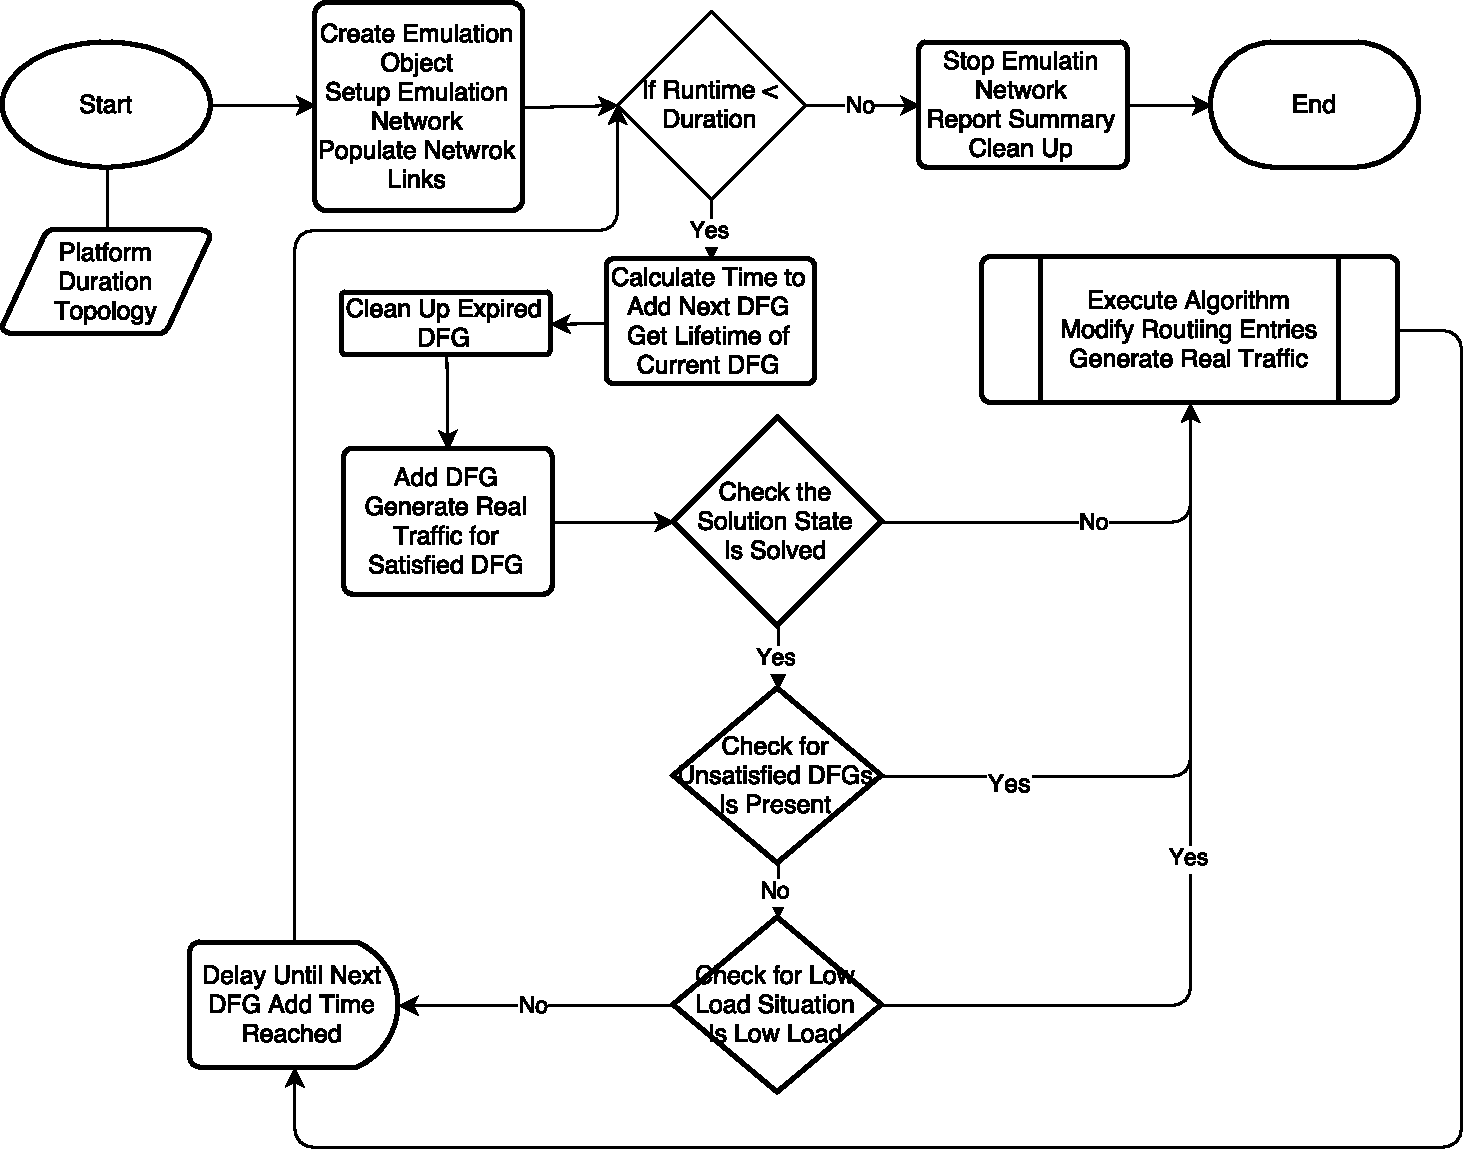
\includegraphics{emulation-flowchart.pdf}}
	\caption{Emulation flow chart.}
	\label{fig:emulationflow}
\end{center}
\end{figure}

The emulation starts with three input parameters, the emulation platform (Mininet or MaxiNet), the duration (how long the emulation will be executed) and the testbed topology description file. First, it creates an emulation object which is basically an object of class \textit{CPFlex}, which prepare the network model reading the topology description file. Then, it set up the network by calling the method \textit{setupEmulationNetwork} (see Section \ref{sec:setnet}); it uses the network model and set up the real network testbed based on specified emulation platform. The method \textit{populateNetworkLinks} (see Section \ref{sec:mrt}) is used to populate the network links information. After which, it starts the loop of the emulation for the specified amount of time the emulation needs to run. Inside the loop, it first calculates a period of time to add the next DFG in the system. I call that period of time $\Delta t$, in that $\Delta t$ the emulation executes following steps:
\begin{itemize}
	\item It handles the blacklisted flows (if any) and remove all the flows which have already expired. Blacklisted flows are those which are on the system but could not be satisfied with the available resources. Therefore, they are blacklisted for a short period of time so that the algorithm does not fall into a loop of repeatedly trying to satisfy them unsuccessfully.
	\item It adds a new DFG in the system and starts real traffic generation for the same. It is important to remember that FlexFCAPF tries to satisfy the DFG when it is added to the system.
	\item It checks if there are any unsatisfied, non-blacklisted DFGs in the network and if there are still unsatisfied DFGs, the emulation set a boolean for executing FlexFCAPF algorithm for the reason of ``Unsatisfied flow in the system".
	\item It moves on and checks for low load situation, if there is no unsatisfied, non-blacklisted DFGs. For low load situation, it tries to remove the lowest loaded LCA from the system and set a boolean to execute FlexFCAPF algorithm with the reason of ``Low Load Situation" to reassign the DFGs and nodes which were assigned to the removed LCA.
	\item If the boolean for executing FlexFCAPF is set, the emulation execute the algorithm. Every time FlexFCAPF algorithm has been executed, there might be a change in the node to LCA assignment, therefore the emulation modifies the routing entries in the underlying network to accommodate that changes via REST API call to the SDN controller. It also configures traffic control objects in the LCAs to introduce delay in the interfaces and starts iperf to generate traffic for all the newly satisfied flows due to resignment.
\end{itemize}
If the emulation could finish all the steps before the $\Delta t$ system time then it sleeps for the remaining time, otherwise, it goes for next iteration of executing above steps. Finally, when the specified emulation duration is reached, it ends the loop, stop the network and do the cleanup.
